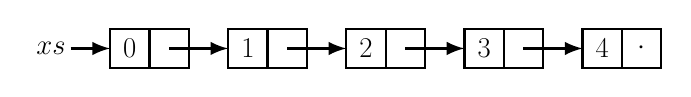
\begin{tikzpicture}[thick,scale=0.5, every node/.style={scale=0.5}]
    \tikzstyle{marrs}=[very thick,-latex]

    \begin{scope}
    
        \foreach \x/\y in {0/0, 3/0, 6/0, 9/0, 12/0} {
            \draw (\x - 0.5, \y - 0.5) rectangle +(1, 1); \draw (\x + 1 - 0.5, \y - 0.5) rectangle +(1, 1);
        }
        \draw[marrs] (-1.5, 0) -> +(1, 0);
        \foreach \x in {1, 4, 7, 10} {
            \draw[marrs] (\x, 0) -> +(1.5, 0);
        }
        
        { \huge
            \draw (-2, 0) node {$xs$};
            \foreach \x/\y in {0/0, 3/1, 6/2, 9/3, 12/4} {
                \draw (\x, 0) node {$\y$};
            }
            \draw (13, 0) node {$\cdot$};
        }
    
    \end{scope}
    
\end{tikzpicture}